En este apartado se define el diseño de las clases que componen el sistema desarrollado. 
En primer lugar, se presenta el diagrama de paquetes, que muestra la estructura de los paquetes que componen el sistema.
Posteriormente, se presenta el diagrama de clases, que muestra las clases que componen el sistema y las relaciones entre ellas así como una descripción.

\subsection{Diagrama de paquetes} 
El sistema se divide en dos paquetes principales:
\begin{itemize}
    \item \textbf{restapi}: se corresponde con el \textit{backend} del sistema, contiene las clases que implementan la API REST del sistema y la lógica de negocio.
    \item \textbf{frontend}: se corresponde con el \textit{frontend} del sistema, contiene las clases que implementan la interfaz de usuario.
\end{itemize}

En la \coloredUnderline{\hyperlink{fig:6_5_Diagrama-Paquetes}{Figura \ref*{fig:6_5_Diagrama-Paquetes}: \nameref*{fig:6_5_Diagrama-Paquetes}}} se muestra el diagrama de paquetes del sistema.
\begin{figure}[H]
    \hypertarget{fig:6_5_Diagrama-Paquetes}{}
    \centering
    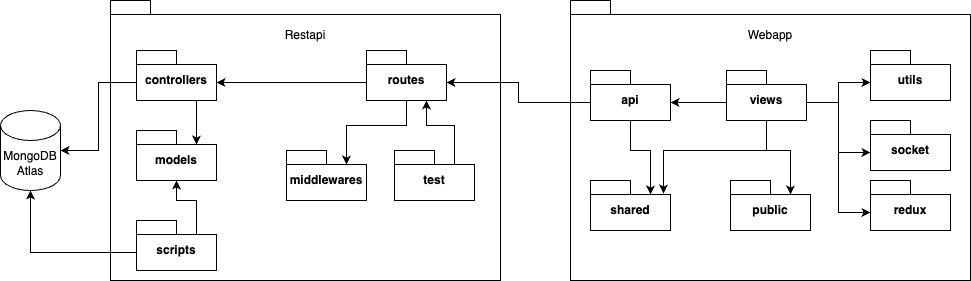
\includegraphics[width=0.8\linewidth]{figures/6-Analisis/6-Clases/6_5-vista_general-paquetes.png}
    \caption{Diagrama de Paquetes del Sistema}
    \label{fig:6_5_Diagrama-Paquetes}
\end{figure}

\subsection{Descripción de los Paquetes}
\subsubsection{restapi}
El paquete \textbf{restapi} contiene las clases que implementan la API REST del sistema y la lógica de negocio. Este paquete se divide en los siguientes subpaquetes:
\begin{itemize}
    \item \textbf{controllers}: contiene las clases que implementan los controladores de la API REST, se encargan de gestionar las peticiones HTTP y las respuestas. Se comunica con la base de datos.
    \item \textbf{models}: contiene las clases que implementan los modelos de datos del sistema.
    \item \textbf{routes}: contiene las clases que implementan las rutas de la API REST, se encargan de definir las rutas y los métodos HTTP asociados.
    \item \textbf{middlewares}: contiene las clases que implementan los middlewares de la API REST, se encargan de gestionar la autenticación y la autorización de los usuarios.
    \item \textbf{scripts}: contiene las clases que implementan los scripts de inicialización de la base de datos.
    \item \textbf{tests}: contiene las clases que implementan las pruebas unitarias de las clases de los otros subpaquetes.
\end{itemize}


\subsubsection{frontend}
El paquete \textbf{frontend} contiene las clases que implementan la interfaz de usuario. Este paquete se divide en los siguientes subpaquetes:
\begin{itemize} 
    \item \textbf{src}: contiene las clases que implementan la lógica de la interfaz de usuario.
    \begin{itemize}
        \item \textbf{api}: contiene las clases que implementan la API del frontend, se encargan de gestionar las peticiones HTTP/HTTPS al backend.
        \item \textbf{views}: contiene las clases que implementan las vistas de la interfaz de usuario. A su vez, se divide en los siguientes subpaquetes:
        \begin{itemize}
            \item \textbf{components}: contiene las clases que implementan los componentes de la interfaz de usuario.
            \item \textbf{pages}: contiene las clases que implementan las páginas de la interfaz de usuario.
        \end{itemize}
        \item \textbf{redux}: contiene las clases que implementan los estados de Redux.
        \item \textbf{socket}: contiene las clases que implementan la conexión con Socket.io.
        \item \textbf{shared}: contiene las clases que implementan los tipos de datos compartidos entre las distintas partes de la interfaz de usuario.
        \item \textbf{utils}: contiene las clases que implementan utilidades de la interfaz de usuario.
    \end{itemize}
    \item \textbf{public}: contiene los archivos estáticos de la interfaz de usuario.
    \item \textbf{tests}: contiene las clases que implementan las pruebas de la interfaz de usuario.
\end{itemize}

\subsection{Diagrama de Clases} 

\subsection{Descripción de las Clases}

